\chapter{Prototypische Implementierung einer Augmented Reality Applikation zur Steuerung eines Roboters}\label{chap:appImplementation}
Dieses Kapitel beschäftigt sich mit der prototypischen Implementierung einer \textit{Augmented Reality} Applikation, die als Teleoperator für einen Roboter dient. Es wird auf die Architektur der Anwendung eingegangen, welche sowohl die Assoziationen der einzelnen Systeme aufzeigt, als auch die konkrete Implementierung der Komponenten: \textit{User Interface}, Befehlsvermittlung an den Roboter, Implementierung der Aktionen der Maschine sowie Implementierung der Gesten und Sprachkommandos.
\section{Kalibrierung der Szene}\label{sec:calibrateScene}
Die Kalibrierung der Szene erfolgt über eine manuelle Kalibrierung. Der Anwender setzt mit Hilfe des \textit{Cursors} zwei Punkte an Anfang und Ende der Führungsschiene des Roboters. Die dabei entstehenden Objekte sind gleichzeitig Ankerpunkte für die Translationgeste. Zwischen ihnen kann später das Interaktionsobjekt hin und her bewegt werden. Die Positionen des linken und rechten Ankerpunkts werden gespeichert und der Mittelpunkt der Strecke zwischen ihnen bildet den Ausrichtungspunkt für das \textit{User Interface} \frqq HoloInterface\flqq.
\section{Realisierung der Interaktionen}\label{sec:implementInteractions}
Die Interaktionen werden mit Hilfe des \textit{HoloToolkit} realisiert. Es bietet Schnittstellen für alle vorgestellten Gesten. Der weitere Vorgang orientiert sich grob an der \textit{Pipeline} aus Abbildung~\ref{fig:pipeline}.

Startet man die Applikation und durchläuft die Kalibrierungsszene erfolgreich, werden im Hauptobjekt der Steuerungsszene, welches den simplen Namen \frqq Manager\flqq\ trägt, die Raum-, Sprach- und Gestenerkennung registriert sowie der \textit{Wrapper} für die EV3-Kommunikationsbibliothek gestartet. Sie wurden jeweils in die Skripte \frqq Voice\flqq-, \frqq Gesture\flqq- und \frqq EV3\flqq-Manager modularisiert.
\subsection{User Interface}\label{ssec:userInterface}
Das \textit{User Interface} wurde ebenfalls nach den, bereits aus Sektion~\ref{ssec:msHoloLens} bekannten, \frqq ASSEFIL-Kriterien\flqq\ als \textit{Wireframe} gestaltet. Der Entwurf dazu ist in Abbildung \ref{fig:holo_interface_wireframe} zu sehen.
\begin{figure}[H]
	\centering
	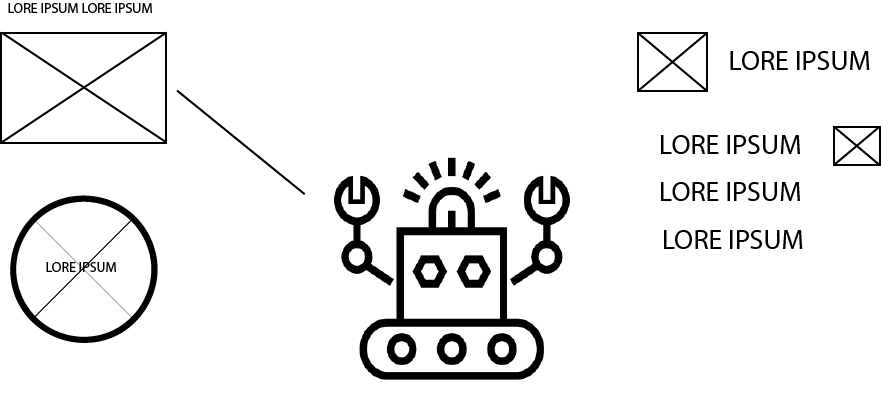
\includegraphics[width=1.0\textwidth]{figuren/InterfaceWireframe}
	\caption{HoloInterface -- \textit{Userinterface} als \textit{Wireframe} Entwurf. Bildquelle: Eigenes Werk.}
	\label{fig:holo_interface_wireframe}
\end{figure}
Er wurde in Anbetracht dessen gestaltet, dass ein Anwender die wichtigsten Informationen den Roboter betreffend während der Interaktion mit ihm vor sich in einem \textit{Headup-Display} wahrnehmen kann, ohne dabei zu sehr von seiner Aufgabe abgelenkt zu werden.
\begin{figure}[H]
	\centering
	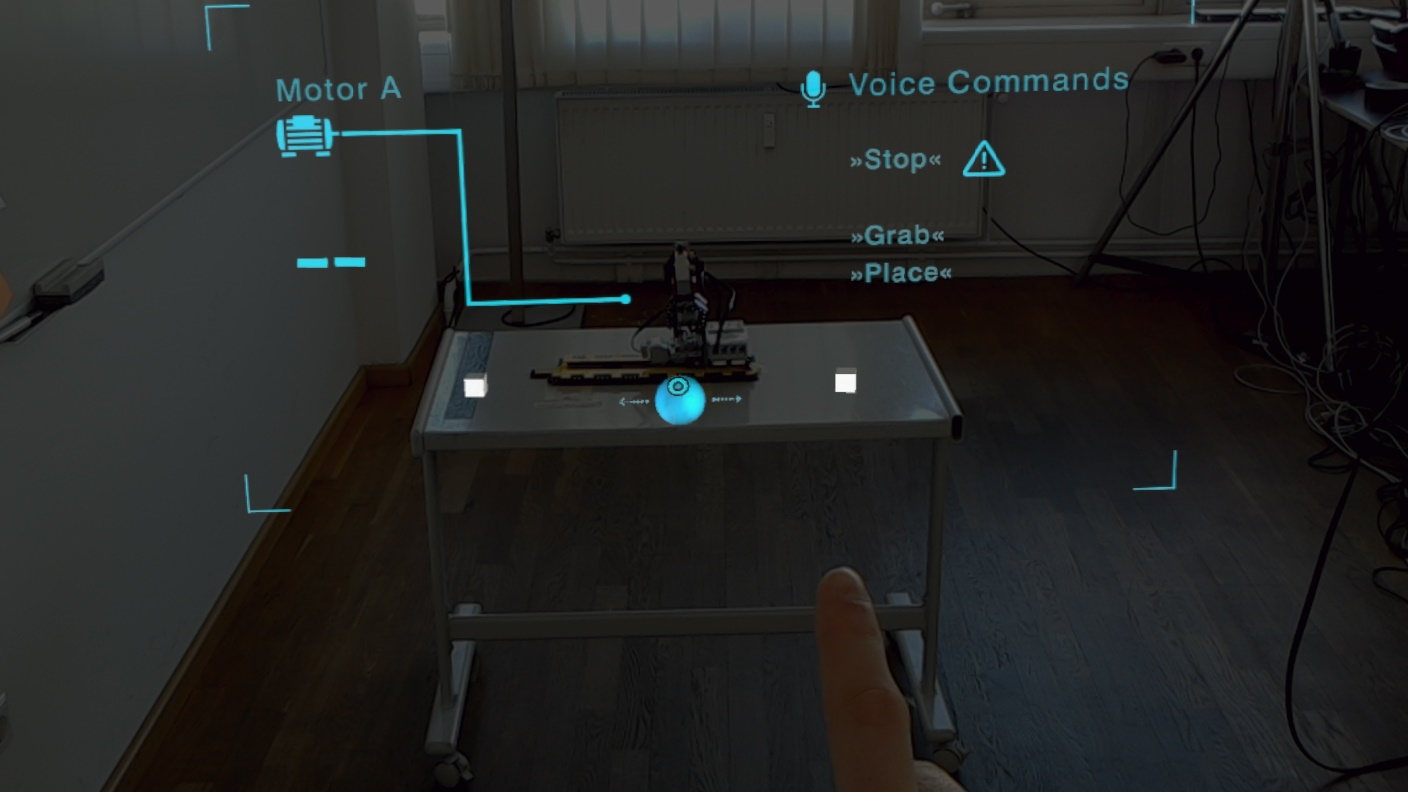
\includegraphics[width=1.0\textwidth]{figuren/HoloInterface}
	\caption{HoloInterface -- \textit{User Interface} für die Applikation \frqq EV3ControllAR\flqq. Bildquelle: Eigenes Werk.}
	\label{fig:holo_interface}
\end{figure}
Das \textit{User Interface} beinhaltet die wichtigsten Informationen auf einen Blick. Zu den essentiellen Informationen zählen: Wie schnell sich \frqq MotorA\flqq\ dreht. Wobei das Vorzeichen die Drehrichtung des Motors anzeigt und dabei angibt, ob der Roboter auf seiner Schiene nach rechts oder links fährt. Zusätzlich wird eine Liste der Sprachkommandos angezeigt, die der Anwender benötigt, um den Greifarm des Roboters zu kontrollieren. Es wurde das HCI-Kriterium \textit{Chunking} beachtet, welches vorgibt, nicht mehr als sieben Elemente in einer Gruppierung zu platzieren, da das menschliche Gehirn nur maximal sieben \textit{Chunks} gleichzeitig aufnehmen kann.\footnote{ Vgl. Gobet / Fernand / Lane et al., S. 236 ff., 2001.}
\subsection{Befehlsvermittlung an die Maschine}\label{ssec:commandMachine}
Die Befehlsvermittlung an die Maschine wurde mit der Kommunikationsbibliothek \textit{MonoBrick} realisiert. Was \textit{MonoBrick} ist und wie es aufgebaut ist, kann in der Sektion~\ref{ssec:monoBrick} nachgeschlagen werden. \textit{MonoBrick} erlaubt es eine Verbindung zum \textit{EV3}-Baustein über Netzwerk zu realisieren, wenn ein kompatibler \textit{WiFi-Dongle} im \textit{USB-Port} des \textit{EV3}-Baustein  eingesteckt wurde. Allerdings muss der \textit{EV3} zunächst überhaupt in die Lage versetzt werden Befehle von außen zu erhalten und eine TCP/IP (Transmission Control Protocol/Internet Protocol) Verbindung herzustellen:\footnote{ Vgl. MonoBrick, Guides, 2016. [Accessed: 15.01.2017].}
\begin{enumerate}
	\item Mit einem Protokollprogramm (\textit{Wireshark}) auf Port 3015 lauschen, denn der EV3 sendet ungefähr im 10-Sekundentakt eine UDP (User Datagram Protocol) Übertragung.
	\item Diese enthält die Seriennummer des EV3 (siehe Abbildung \ref{fig:wireshark}).
	\item Hat man die Seriennummer notiert, muss man eine beliebige UDP-Nachricht an den EV3 senden.
	\item Danach ist der Stein bereit TCP/IP-Nachrichten zu empfangen.
	\item Jetzt folgt die Freigabe-Nachricht via TCP/IP:
	\begin{itemize}
		\item GET /target?sn=0016534e474f VMTP1.0 Protocol: EV3 
	\end{itemize}
	\item Antwortet der Stein mit einer 16 Byte langen TCP/IP-Nachricht mit dem Inhalt Accept:EV340 ist der Stein freigeschaltet und der obige Code lässt die Kommunikation zwischen EV3 und Applikation via TCP/IP zu.
\end{enumerate}
\begin{figure}[H]
	\centering
	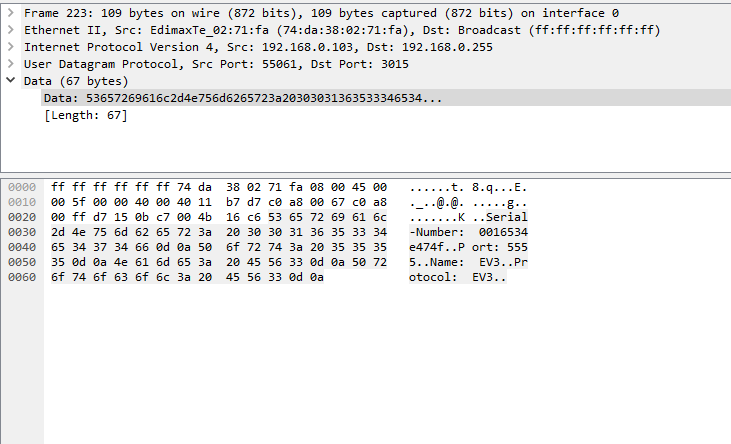
\includegraphics[width=.75\textwidth]{figuren/wireshark}
	\caption{UDP-Paket des \textit{EV3} im Netzwerk, welches die Seriennummer enthält. Bildquelle: Eigenes Werk.}
	\label{fig:wireshark}
\end{figure}
Ist erst einmal eine Verbindung geöffnet und initialisiert, kann mit dem \textit{EV3}-Baustein über die Schnittstelle von \textit{MonoBrick} kommuniziert werden.
Folgender Codeabschnitt zeigt die Deklaration, Initialisierung und Aktivierung der Verbindung zwischen dem \textit{EV3} und der \textit{Wrapper}-Klasse \frqq EV3-Manager\flqq\ mit Hilfe der \textit{MonoBrick}-Kommunikationsbibliothek:\\
\begin{lstlisting}
using UnityEgine;
using MonoBrick.EV3;

public class EV3Manager : MonoBehaviour {
	
	public Brick<TouchSensor, Sensor, Sensor, Sensor>; 
	[...]
	
	void Start() {
		ev3 = new Brick<TouchSensor, Sensor, Sensor, Sensor>("WiFi");
		ec3.Connection.Open();
		[...]
	}
	[...]
}
\end{lstlisting}
Die Bewegungsabfolgen des \textit{EV3} wurden ebenfalls im \textit{EV3-Manager} implementiert. Sie orientieren sich an den vier \textit{User Stories} aus Sektion \ref{ssec:usecase}.

\paragraph*{MoveRobot} Übermittelt die Geschwindigkeit des MotorsA, welcher für die Translation auf der Schiene zuständig ist als Wert vom Typ \textit{sbyte}. Die Methode kann einen Wert zwischen -100 und 100 annehmen, was die maximale Geschwindigkeit des Servomotors in beide Richtungen angibt.

\begin{lstlisting}
public void MoveRobot(sbyte speed) {
  ev3.MotorA.On(speed);     
}
\end{lstlisting}

\paragraph*{ExecuteGrab} Beläuft sich auf drei Aktionen des Roboterarms: Den Arm nach unten bewegen; Greifer schließen; Arm nach oben bewegen. Wird dann der Berührungssensor am Roboterarm aktiviert hält der Arm seine Position.

\begin{lstlisting}
public void GrabObject() { 
  WaitForMotorToStop();         
  ev3.MotorB.Off();         
  WaitForMotorToStop();         
  ev3.MotorC.MoveTo(10, 80, true);         
  WaitForMotorToStop();         
  ev3.MotorB.On(-25);         
  MotorBlocked = true;     
}
\end{lstlisting}

Die \textit{Update}-Methode prüft dabei den Zustand des Berührungssensors.

\begin{lstlisting}
if (ev3.Sensor1.Read() == 1 && MotorBlocked == true) { 
  ev3.MotorB.Brake();             
  MotorBlocked = false;
}
\end{lstlisting}

\paragraph*{PlaceObject} Diese Methode verhält sich analog zur \textit{Grab}-Methode und bedarf keiner weiterer Erklärung.

\paragraph*{EmergencyStopp} Die Methode stoppt sofort alle Motoren und lässt den Roboter in seiner Position verharren.

\begin{lstlisting}
  ev3.MotorA.Off();
  ev3.MotorB.Off();
  ev3.MotorC.Off(); 
\end{lstlisting}
\subsection{Implementierung der Gesten}\label{ssec:gestureCommands}
Gesten sind, wie in Kapitel aufgezeigt, eine der drei Hauptformen, um mit Hologrammen zu interagieren. Zunächst muss jedoch ein Hologramm anvisiert werden. In der Applikation \textit{EV3ControllAR} ist dafür der \textit{GazeManager} verantwortlich. Er generiert einen \textit{Raycast}\footnote{ Raycasting ist der Prozess des Schießens eines unsichtbaren Strahls von einem Punkt aus in eine spezifische Richtung und des Detektierens von Schnittpunkten des Strahls mit \textit{Collidern} in der Szene.}, welcher aus der Mitte der Datenbrille abgefeuert wird und somit der Kopfbewegung und im weiteren Sinne dem Blick des Trägers folgt. Wurde ein Hologramm mit dem \textit{Cursor} anvisiert, wird die Position und Normale des vom \textit{Raycast} des \textit{Cursors} getroffenen \textit{GameObjects} zurückgegeben und die Ergebnisse können weiterverarbeitet werden. Folgender Codeauschnitt aus Anhang~\ref{code:GazeManager} zeigt die Implementierung des \textit{Cursors}:
\begin{lstlisting}
[...]
  gazeOrigin = Camera.main.transform.position;
  gazeDirection = Camera.main.transform.forward;
  gazeStabilizer.UpdateHeadStability(gazeOrigin, Camera.main.transform.rotation);
  gazeOrigin = gazeStabilizer.StableHeadPosition;
  UpdateRaycast();
			
  /// <summary>
  /// Calculates the Raycast hit position and normal.
  /// </summary>         
  private void UpdateRaycast() {
	RaycastHit hitInfo;
	Hit = Physics.Raycast(gazeOrigin, gazeDirection, out hitInfo, MaxGazeDistance, RaycastLayerMask);
	HitInfo = hitInfo;
	if (Hit) { // If raycast hit a hologram...
	  Position = hitInfo.point;
	  Normal = hitInfo.normal;
	}
[...]
\end{lstlisting}
Wurde ein Hologramm getroffen, ist es sinnvoll, die Gestalt des \textit{Cursors} zu ändern und eine Nachricht an das getroffene Hologramm zu senden, sodass der Benutzer ein \textit{User Feedback} bekommt, welches weitere Aktionsmöglichkeiten visualisiert sowie Befehle an das getroffene Hologramm gesendet werden können. Dafür zuständig sind die Skripte \textbf{InteractibleManager} und \textbf{CursorManager} sowie \textbf{Interactible}. Die Hauptaufgabe des \textit{InteractibleManager}s ist es ein \textit{GameObject} zu erstellen und dieses mit der \textit{hitInfo} des \textit{GazeManager}s anzureichern. Die folgenden Codeabschnitte zeigen dieses Verhalten und beleuchten kurz die Änderung des \textit{Cursor-Icons}. Wie im Anhang~\ref{code:CursorManager} ab Zeile 29 zu sehen, entscheidet diese Klasse darüber, welcher \textit{Cursor} aktiv sein soll, basierend darauf, ob ein Hologramm getroffen wird oder nicht. Des Weiteren übernimmt sie das setzen der \textit{Cursor}-Position:
\begin{lstlisting}
[...]
if (GazeManager.Instance == null || CursorOnHolograms == null || CursorOffHolograms == null) {
	return;
}

if (GazeManager.Instance.Hit) {
	CursorOnHolograms.SetActive(true);
	CursorOffHolograms.SetActive(false);
} else {
	CursorOffHolograms.SetActive(true);
	CursorOnHolograms.SetActive(false);
}
	
gameObject.transform.position = GazeManager.Instance.Position;
	
gameObject.transform.up = GazeManager.Instance.Normal;
[...]
\end{lstlisting}
Der Codeausschnitt aus Anhang~\ref{code:InteractibleManager} ist für das Umschalten des Cursors und das Senden von Nachrichten an das getroffene \textit{GameObject} zuständig.
\begin{lstlisting}
[...]
if (hitInfo.collider != null) {
  /// Assign the hitInfo's collider gameObject to the FocusedGameObject.
  FocusedGameObject = hitInfo.collider.gameObject;
}
[...]
if (FocusedGameObject != null) {
  if (FocusedGameObject.GetComponent<Interactible>() != null) {
  /// Send a GazeEntered message to the FocusedGameObject.
  FocusedGameObject.SendMessage("GazeEntered");
  }
}

private void ResetFocusedInteractible() {
  if (oldFocusedGameObject != null) {
	if (oldFocusedGameObject.GetComponent<Interactible>() != null) {
	  /// Send a GazeExited message to the oldFocusedGameObject.
	  oldFocusedGameObject.SendMessage("GazeExited");
	}
  }
}
[...]
\end{lstlisting}
Ist der \textit{Cursor} und dessen Verhalten implementiert, folgt als nächstes die Gestenerkennung. Zur Gestenerkennung gehören die Skripte \textbf{HandsManager}, \textbf{GestureManager} und \textbf{GestureAction}. Im \textit{Handsmanager} meldet man die Ereignisse \textit{SourceDetected} und \textit{SourceLost} mit folgenden Codezeilen an und wechselt das \textit{Cursor-Asset} dementsprechend aus:
\begin{lstlisting}
[...]
InteractionManager.SourceDetected += InteractionManager_SourceDetected;
InteractionManager.SourceLost += InteractionManager_SourceLost;

/// Register for SourceManager.SourcePressed event.
InteractionManager.SourcePressed += InteractionManager_SourcePressed;

/// Register for SourceManager.SourceReleased event.
InteractionManager.SourceReleased += InteractionManager_SourceReleased;

[...]
private void InteractionManager_SourceDetected(InteractionSourceState hand) {
  HandDetected = true;
}

private void InteractionManager_SourceLost(InteractionSourceState hand) {
  HandDetected = false;
  ResetFocusedGameObject();
}
\end{lstlisting}
Danach wird im \textit{GestureManager} festgelegt, welche Gesten erkannt werden sollen; in Fall von \textit{EV3ControllAR} Applikation sind das die Navigation auf X-Ebene zur Verschiebung des Interaktionselements und die \textit{Tap}-Geste:
\begin{lstlisting}
/// Instantiate the NavigationRecognizer.
NavigationRecognizer = new GestureRecognizer();

/// Add Tap and NavigationX GestureSettings to the NavigationRecognizer's RecognizableGestures.
NavigationRecognizer.SetRecognizableGestures(GestureSettings.Tap | GestureSettings.NavigationX);
\end{lstlisting}
Das an das Interaktionsobjekt angehängte Skript \textit{GestureAction} behandelt den Sachverhalt, dass der Roboter bewegt werden soll, wann immer das Interaktionsobjekt translatiert wird. Dazu rechnet man den Translationsfaktor in die Handbewegung ein und überträgt eine daraus passende Geschwindigkeit an den Motor des Roboters, welcher für die Lokomotion zuständig ist; wird während der Translation die Navigationsgeste unterbrochen, stoppt der Roboter.
\begin{lstlisting}
[...]
public float TranslationSensitivity = 10.0f;
private float translationFactor;   
[...]    

void Update(){      
  PerformTranslation();   
}     

private void PerformTranslation() {         
  if (GestureManager.Instance.IsNavigating && HandsManager.Instance.FocusedGameObject == gameObject) {             
	// Calculate translationFactor based on GestureManager's NavigationPosition.X and multiply by TranslationSensitivity.             
	// This will help control the amount of translation.             
	translationFactor = GestureManager.Instance.NavigationPosition.x;          

	// Restrict the translationFactor to a value between -1 and 1, so the robot doesn't get to fast.
	float clampTranslation = Mathf.Clamp(translationFactor, -1f, 1f);      
	positionManager.SetPosition(clampTranslation / 2 + 0.5f);
	ev3.MoveRobot((sbyte)(clampTranslation * 10));         
  } else {             
	positionManager.SetPosition(0.5f);             
	ev3.StopRobot();         
  }     
} 
\end{lstlisting}
Zusätzlich wurden Sprachkommandos implementiert, die den Greifarm des Roboters steuern. Sie werden zusammen mit ihrer Implementation genauer in der nächsten Sektion \ref{ssec:voiceCommands} behandelt.
\subsection{Implementierung der Sprachkommandos}\label{ssec:voiceCommands}
Drei der vier Anwendungsfälle wurden mit Sprachkommandos realisiert: Dabei handelt es sich um die Anwendungsfälle \textit{GrabObject} aus Tab. \ref{tab:usecase2}, \textit{PlaceObject} aus Tab. \ref{tab:usecase3} sowie \textit{Stop} aus Tab. \ref{tab:usecase4}. Die Realisierung von Sprachbefehlen in \textit{Unity} kann auch drei Art und Weisen gestaltet werden: \begin{enumerate}
	\item PhraseRecognizer
	\item GrammaerRecognizer
	\item DictationRecognizer
\end{enumerate}
Bei der vorliegenden Arbeit wurde der \textit{KeywordRecognizer} als Spracheingabe gewählt und im Skript \textbf{VoiceManager} implementiert, da er sich für die Anwendungsfälle, welche klare Befehle an eine Maschine übertragen sollen, am besten eignet, da nur einzelne Schlüsselwörter erkannt und auf diese reagiert werden soll.
Zunächst muss spezifiziert werden, auf welche Schlüsselwörter der \textit{KeywordRecognizer} hören soll und die Aktion definiert werden, die nach Erkennung durchgeführt werden soll. Folgender Code aus Anlage~\ref{code:VoiceManager} ist dafür zuständig.
\begin{lstlisting}
[...]
/// Initialize...
KeywordRecognizer keywordRecognizer;
Dictionary<string, System.Action> keywords = new Dictionary<string, System.Action>();
[...]
/// Create keywords and add them to dictionary...
keywords.Add("grab", () => {             
  ev3.GrabObject();
});
keywords.Add("place", () => {             
  ev3.PlaceObject();
});
keywords.Add("stop", () => {             
  ev3.Stop();
});
[...]
/// Tell KeywordRecognizer which words to recognize.
keywordRecognizer = new KeywordRecognizer(keywords.Keys.ToArray());
/// Register for OnPhraseRecognized event
keywordRecognizer.OnPhraseRecognized += KeywordRecognizer_OnPhraseRecognized;
/// Start recognizing...    
keywordRecognizer.Start();

private void KeywordRecognizer_OnPhraseRecognized(PhraseRecognizedEventArgs args) {
  Debug.Log("Keyword Recognized..." + args.text);
  System.Action keywordAction;
  /// Fire action depending on which keyword was recognized.
  if (keywords.TryGetValue(args.text, out keywordAction)) {
	keywordAction.Invoke();
  }
}
\end{lstlisting}